\documentclass{cslesson}
\usepackage[cache=false]{minted}

\usepackage{tikz}
\usetikzlibrary{positioning,shapes,fit,arrows}
\definecolor{myblue}{RGB}{56,94,141}

\title{Basic OOP in Python}
\author{SLSS Computer Science Club}
\date{September 21, 2018}

\begin{document}

\maketitle

Up until now, all the programs that we have wrote have been strictly procedural in nature; that is, we have designed our programs
such that they are structured around functions and scopes that manipulate data. This method of programming or \textit{paradim} is known
as \textit{procedural programming}. However, there exist other ways of structuring our programs. In this lesson, we will discuss the
\textit{object-oriented programming} paradigm which organizes the program in structural blocks of data that contain logic or \textit{functionality}. 
In simpler terms, object-oriented programming focuses on treating data as objects with properties and logic that operates on these properties rather than 
imperative commands.

Oftentimes, for small applications (e.g. contest programming), procedural programming is preferable to the object-oriented programming paradigm. However,
when writing large applications, object-oriented techniques are recommend as they lead to better structured programs with code that is cleaner and 
more maintainable. 

\section{Why Take the Object-Oriented Approach?}

Before we study object-oriented programming, let's explore some of the flaws with procedural programming
and how we can solve these issues using object-oriented programming.

Suppose we are creating a program and we need to represent many circles: their $(x,y)$ position and radius. An obvious and simple approach
would be to create three lists $X$, $Y$, and $R$ that hold the $x$-position, $y$-position, and radius of the circle respectively. For a circle $C_i$, $X_i$
represents the $x$-position of $C_i$, $Y_i$ represents the $y$-position of that circle, and $R_i$ represents the radius. Thus, (ideally) all lists have the 
same length, or mathematically, $\left|X\right|=\left|Y\right|=\left|R\right|=n$ where $n$ is the amount of circles. To store the information
about a new circle $C_j$, we would insert the $x$-position of $C_j$ into $X$, insert the $y$-position into $Y$, and insert the radius into $R$:
\begin{minted}[frame=lines,framesep=2mm]{python}
    x_positions = []
    y_positions = []
    radii =  []
    
    # ...
    # Add circle at (5,6) with radius of 10
    
    x_positions.append(5)
    y_positions.append(6)
    radii.append(10)
        
\end{minted}

Of course, suffice to say, this ``solution'' is \textit{very} bad;
one of the biggest flaws is the fact that there is nothing to stop the lists from going out of sync with one another. Specifically, there is no 
mechanism to stop an unaware programmer from inserting or removing an element from one of the lists. Even worse, due to the fact that the information
about a circle is mapped by index across three arrays, if an element is removed from one of the lists, all the other elements now have an index
that is referring to the wrong circle. Figure \ref{fig:out_of_sync_array} shows how a list might become out of sync when an element is removed.

\begin{figure}[h]
    \centering
    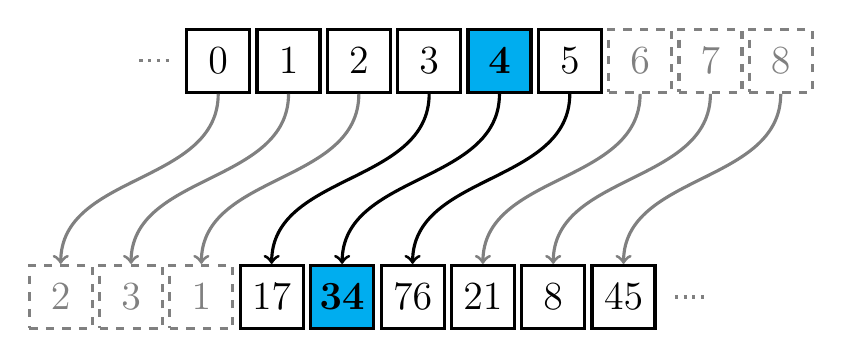
\begin{tikzpicture}
        \def\boxgap{+0.053cm}
        \def\minboxsz{0.8cm}
        \def\boxlinewidth{0.04cm}
         
        \draw[gray, dotted, line width=0.04cm] (1, 3) -- (1.4, 3);
        \node[rectangle, draw, line width=\boxlinewidth, minimum size=\minboxsz] (a1) at (2, 3) {\Large 0};
        \node[rectangle, draw, line width=\boxlinewidth, minimum size=\minboxsz, right = \boxgap of a1] (b1) {\Large 1};
        \node[rectangle, draw, line width=\boxlinewidth, minimum size=\minboxsz, right = \boxgap of b1] (c1) {\Large 2};
        \node[rectangle, draw, line width=\boxlinewidth, minimum size=\minboxsz, right = \boxgap of c1] (d1) {\Large 3};
        \node[rectangle, draw, line width=\boxlinewidth, minimum size=\minboxsz, right = \boxgap of d1, fill=cyan] (e1) {\Large \textbf{4}};
        \node[rectangle, draw, line width=\boxlinewidth, minimum size=\minboxsz, right = \boxgap of e1] (f1) {\Large 5};
        \node[rectangle, draw, line width=\boxlinewidth, minimum size=\minboxsz, right = \boxgap of f1, dashed, gray] (g1) {\Large \textcolor{gray}{6}};
        \node[rectangle, draw, line width=\boxlinewidth, minimum size=\minboxsz, right = \boxgap of g1, dashed, gray] (h1) {\Large \textcolor{gray}{7}};
        \node[rectangle, draw, line width=\boxlinewidth, minimum size=\minboxsz, right = \boxgap of h1, dashed, gray] (i1) {\Large \textcolor{gray}{8}};
         
        \node[rectangle, draw, line width=\boxlinewidth, minimum size=\minboxsz, dashed, gray] (x2) at (0, 0) {\Large \textcolor{gray}{2}};
        \node[rectangle, draw, line width=\boxlinewidth, minimum size=\minboxsz, right = \boxgap of x2, dashed, gray] (y2) {\Large \textcolor{gray}{3}};
        \node[rectangle, draw, line width=\boxlinewidth, minimum size=\minboxsz, right = \boxgap of y2, dashed, gray] (z2) {\Large \textcolor{gray}{1}};
        \node[rectangle, draw, line width=\boxlinewidth, minimum size=\minboxsz, right = \boxgap of z2] (a2) {\Large 17};
        \node[rectangle, draw, line width=\boxlinewidth, minimum size=\minboxsz, right = \boxgap of a2, fill=cyan] (b2) {\Large \textbf{34}};
        \node[rectangle, draw, line width=\boxlinewidth, minimum size=\minboxsz, right = \boxgap of b2] (c2) {\Large 76};
        \node[rectangle, draw, line width=\boxlinewidth, minimum size=\minboxsz, right = \boxgap of c2] (d2) {\Large 21};
        \node[rectangle, draw, line width=\boxlinewidth, minimum size=\minboxsz, right = \boxgap of d2] (e2) {\Large 8};
        \node[rectangle, draw, line width=\boxlinewidth, minimum size=\minboxsz, right = \boxgap of e2] (f2) {\Large 45};
        \draw[gray, dotted, line width=0.04cm] (7.8, 0) -- (8.2, 0);
         
        \draw [->, line width=0.04cm, gray] (a1) to[out=270, in=90] (x2);
        \draw [->, line width=0.04cm, gray] (b1) to[out=270, in=90] (y2);
        \draw [->, line width=0.04cm, gray] (c1) to[out=270, in=90] (z2);
        \draw [->, line width=0.04cm] (d1) to[out=270, in=90] (a2);
        \draw [->, line width=0.04cm] (e1) to[out=270, in=90] (b2);
        \draw [->, line width=0.04cm] (f1) to[out=270, in=90] (c2);
        \draw [->, line width=0.04cm, gray] (g1) to[out=270, in=90] (d2);
        \draw [->, line width=0.04cm, gray] (h1) to[out=270, in=90] (e2);
        \draw [->, line width=0.04cm, gray] (i1) to[out=270, in=90] (f2);
    \end{tikzpicture}
    \label{fig:out_of_sync_array}
    \caption{An out of sync list caused by the removal of an element.}
\end{figure}

Another approach to storing the circles would be to use a nested list; that is, a list of lists which contain the circle information ($x,y$ position and radius):
\begin{minted}[frame=lines,
    framesep=2mm]{python}
    circles = []

    # ...
    # Add circle at (5,6) with radius of 10

    # list = [x, y, radius]
    circles.append([5, 6, 10])
\end{minted}
However, managing this list is still troublesome and the values stored in the secondary list are ambiguous.

Instead, what we seek is an individual method of storing the data required to represent a circle. 
Object-oriented programming enables us to do this using two fundamental concepts: 
\textit{classes} and \textit{objects}.

\section{Introduction to Concepts and Terminology}

In object-oriented programming, classes are at the core of the paradigm.\footnote{Quite literally, without classes, there is no OOP.} 
A class is something that both \textit{encapsulates} data and contains \textit{methods} which can operate on that data. 
As an example, the \texttt{str} class stores a string of characters as its data and contains a \texttt{str.upper()} method which operates 
on the string data. We also use the term \textit{object} or \textit{instance} to refer to an instance of a class. 
For example, the integer 17 is an instance of the \texttt{int} data type (or class) in Python.

Variables that belong to an object or class are called fields. Furthermore, a method is a function that is part of a class. 
This distinction in terminology allows us to differentiate between independent functions and variables and ones which belong to an object. 
The fields and methods of the class are called \textit{attributes} or \textit{members} of the class or object. There are two types of attributes---ones 
which belong to an instance of the object and ones which belong to the object itself. They are called \textit{instance} attributes and \textit{class} 
attributes respectively.

Classes can also contain additional functionality. For example, we are able to concatenate (combine) two strings using the \texttt{$+$} operator
using the built-in addition function. These built-in functions are \textit{special methods} whose names always start and end with a double underscore
and which are provided by the Python interpreter (e.g. \texttt{\_\_add\_\_} or \texttt{\_\_len\_\_}). Thus, by convention, we should never define
an attribute with a number that starts and ends with double underscores.

\section{Classes in Python}

There is one last concept we must explore before beginning to create our own classes: the \texttt{self}. Methods differ from ordinary functions
in only their arguments---they must have an extra first argument at the beginning of the function parameter list. However, when we
call the method, we \textit{do not} give a value to this parameter because Python will provide it for us. This value refers to the instance of the 
object which the method was called from; hence, by convention, the value is called \texttt{self}.\footnote{Technically, we can assign any name to this
parameter but it is \textit{highly recommended} that we use the name \texttt{self} as any other name is not adherent to the convention and is frowned upon
by the Python community}

\subsection*{How Does \texttt{self} Work?}
The \texttt{self} parameter works because of how Python treats methods from the perspective of the interpreter. In reality, Python is all about syntactic sugar
and this is surely no exception. Suppose we have defined a class called \texttt{Foo} and an instance of the class called \texttt{foobar}. When we call a method
on the object such as \texttt{foobar.method(arg1)}, Python converts that into \texttt{Foo.method(foobar, arg1)}. Because of this, even methods with no
arguments must still include \texttt{self} within their parameter list:
\begin{minted}[framesep=2mm]{python}
    # A parameterless method must still include self
    def method(self):
        pass # do nothing
\end{minted}

\subsection{A Simple Class}
We create a new class in Python using the \texttt{class} keyword along with the name of the class. Like a loop or conditional, a class is a block and thus must be
followed by a colon and then an indented block of statements (which form the body of the class):

\begin{minted}[framesep=2mm]{python}
    # A class called foo
    class Foo:
        pass # do nothing
\end{minted}

In the case above, we define a class called \texttt{Foo} with an empty block indicated by the \texttt{pass} statement.

We can create an object or instance of the \texttt{Foo} class by calling the name of class as a function. This is called \textit{instantiating} the class:
\begin{minted}[framesep=2mm]{python}
    # We create an instance of the Foo class
    foobar = Foo()
\end{minted}

We can also add a method to our class. Let's create a method that takes in two numbers as arguments, computes their sums, and then prints the sum:

\begin{minted}[frame=lines, framesep=2mm]{python}
    # A class called foo
    class Foo:
        def sum(self, a, b):
            print(a + b)

    foobar = Foo()
    foobar.sum(2, 2)
    # this script will output 4
\end{minted}

Note, even though we don't use the \texttt{self} variable, we still have to include it in the method parameter list because it is required by Python.

\subsection{Class Constructor}
Earlier we discussed how Python provides many different built-in functions that range in functionality. One of the most important built-in function for classes
is the \texttt{\_\_init\_\_} method.

The \texttt{\_\_init\_\_} method is called as soon as the object is \textit{instantiated} (or created). This method is useful because it allows us to do
any initialization with our object (e.g. passing initial values to our object). In object-oriented programming, this is called the object \textit{constructor}.

Suppose we wanted to have a class that contains the information about a person. We could pass this information into our constructor:

\begin{minted}[frame=lines, framesep=2mm]{python}
    class Person:
        def __init__(self, name):
            self.name = name

        def say(self):
            print('Hi, my name is ' + self.name)

    person = Person('Bob')
    person.say()

    # this script will output 'Hi my name is Bob'
\end{minted}

In the example above, we define the \texttt{\_\_init\_\_} method which takes in a \texttt{name} parameter (along with the required parameter of \texttt{self}).
Then, we create a new field in the \texttt{self} instance called \texttt{name}. In Python, this is how instance attributes are created---by assigning the
assigning the variable as a reference from \texttt{self} (this works because of how the Python language is designed).

Notice how we \textit{do not} explicitly call the \texttt{\_\_init\_\_} method. This is a task that is relegated to the Python interpreter whenever we create
a new instance of the \texttt{Person} class.

\subsection{Variables in Classes}
In classes, they are two types of variables whose distinction relate to the \textit{namespace} 
which they are \textit{bound} with. Fields are simply ordinary variables which are bound to either
the instance or the class itself. When we say a variable is \textit{bound} to a class or object, we mean that the
variables names are only valid in the context of the class or object.

\textit{Class variables} are variables which are bound to the class itself. They can be accessed by all
instances of the class and there exists only one copy of the variable. Because of this, if a class variable
is changed, the change will be seen by all other instances.

\textit{Instance variables} are variables which are bound to an instance of the class; that is, each individual
instance has its own copy of the variable. They are neither shared nor related to another field with the same name
in a different instance. Hence, if an instance variable is changed by one class, the change is not seen by an other instance.

Let's use an example to illustrate the concept better:
\newpage
\begin{minted}[frame=lines, framesep=2mm]{python}
    class Person:
        # The amount of people which exist in the
        # lifetime of the program
        count = 0
        
        def __init__(self, name):
            self.name = name
            Person.count += 1
        
        def destroy(self):
            print('Destroying ' + self.name)
            Person.count -= 1
            Person.get_count()

        @classmethod
        def get_count(cls):
            print('There are ' + str(cls.count) + ' people left')

    people = [
        Person('Bob Sparkles'),
        Person('Justin Findlay'),
        Person('Trevor Lane),
        Person('Steven Pinker')
    ]

    Person.get_count()
    people[0].destroy()

    print('\nPeople left:')
    for person in people:
        print(person.name)
\end{minted}
which outputs:
\begin{minted}[frame=lines, framesep=2mm]{text}
    There are 4 people left
    Destroying Bob Sparkles
    There are 3 people left

    People left:
    Bob Sparkles
    Justin Findlay
    Trevor Lane
    Steven Pinker
\end{minted}

In the example code above, we have two variables: \texttt{population} and \texttt{name} which are class and instance
variables respectively. That is, the \texttt{name} variable belongs in the namespace of the instance and the \texttt{population}
variable belongs in the namespace of the class.

We refer to the \texttt{population} variable as \texttt{Person.population} because it is a class variable. Conversely,
we refer to the \texttt{name} variable as \texttt{self.name} because it is an instance variable. Notice that the difference
between class and instance variables is simply in how we \textit{access} it.

Methods can also belong to the class rather than the instance. In our example, the \texttt{get\_count} is a 
\textit{class method}. We can define class methods using the \textit{classmethod} or \textit{staticmethod} 
decorator. Practically---for our use cases---there is no difference between these two decorators; however, 
by convention, \texttt{classmethod} should be used when the method accesses a class variable and \texttt{staticmethod} 
when it does not.

Another thing to note is that all variables in a class are \textit{public}. This means that we can access the variable
from anywhere within the program. By convention, members of a class which are intended to be private are prefixed
with a double underscore (e.g. \texttt{\_\_privatevar}).

\section{Summary}
Using object-oriented programming, it is now possible for us to efficiently and effortlessly represent a large amount of circles:
\begin{minted}[frame=lines, framesep=2mm]{python}
    import math

    class Circle:
        def __init__(self, x, y, radius):
            self.x = x
            self.y = y
            self.radius = radius

        def area(self):
            return math.pi * self.radius**2

        def distance(self, px, py):
            return math.sqrt((px-self.x)**2 + (py-self.y)**2)

    circles = []

    # ...
    # Add circle at (5,6) with radius of 10

    circle = Circle(5, 6, 10)
    circles.append(circle)
\end{minted}

This lesson covered the basics of object-oriented programming and how it's applications in Python. We explored the concept of classes and objects
and the various terminologies associated with them. We also compared procedural programming to the object-oriented paradigm. 

\end{document}